\chapter{\hspace*{3pt} Methods}
\label{chapter:methodology}

%Automatic text classification consists of automatically assigning a predefined label to textual documents. The use of text classification can be observed in (i) organization through routing, filtering and metadata assignments; (ii) analysis, through the statistics of the labels assigned to the documents or through descriptive and predictive analyzes; and (iii) knowledge extraction, through a set of rules or values that summarize the patterns present in the collection of documents. 
%Moreover, information retrieval engines which correspond to many of the use of the Internet for locating information and gaining knowledge, make use of text classification algorithms to rank the most relevant documents according to a user's query ~\cite{Manning:2008}.

%To perform automatic text classification, expert systems or machine learning algorithms may be used. In the first case, one or more domain experts create a set of conditional rules based on the presence or frequency of a set of words or sentences that define the class of a document. However, manually generated rules are complicated to create or update for different applications or domains and are dependent on the presence and effort of domain experts or knowledge engineers~\cite{Manning:2008}. 

%For that reason, automatic text classification is one of the most studied and used areas to accomplish the tasks mentioned above. 

This chapter presents in detail the steps of the approach applied to the extraction and representation of document features based on the \gls{wcg}.


\section{\hspace*{3pt} Approach} \label{sec:approach}
 
The rich structure of the \gls{wcg} has contributed to making it a large and meaningful semantic taxonomy. The main goal of the research reported on in this thesis is to take advantage of this body of knowledge by automatically categorizing text-based content on the Web following the collective knowledge of Wikipedia contributors. A processing chain to generate a generic categorization was developed based on three steps: 

\begin{enumerate}
\item Text annotation;
\item Categories extraction; and
\item Document Representation.

\end{enumerate}
The relationships between Wikipedia Categories have been considered as a directed graph. Let $G$=($V$, $E$) be a graph, where $V$ is the set of nodes representing Wikipedia categories, and $E$ is the set of edges representing the relationships between them.

For ease of comprehension, the method will be illustrated by way of a running example in a possible real application scenario.
 
 
Imagine that you are the editor of a news site and have received a complex article from the journalist to be published. Your task is to define which categories to attribute to the article so that the content is well represented and allows users to find it on the site quickly. 


As an example for this scenario, let us use an excerpt from the article entitled ``Market Totalitarianism in North Korea", taken from The New York Times\footnote{\url{https://www.nytimes.com/}} of May 3, 2017: \

\textit{"(...) Post-Communist, postindustrial, kleptocratic dynastic regime of North Korea may become the crown jewel of the new axis-of-tyranny ideology (...)"}\footnote{\url{https://nyti.ms/2py3z4r}} \



\subsection{\hspace*{3pt} Text Annotation} 
\label{sec:text-annotation}

Documents on the Web are primarily unstructured data, which hinders data manipulation and the identification of atomic elements in the texts. To alleviate this problem, \gls{ie} methods, such as \gls{ner} are employed. These methods automatically extract structured information from unstructured data and make it possible to link them to external knowledge bases. 

%As described directly on the DBpedia about page
DBpedia describes itself as a ``crowd-sourced community effort to extract structured content from the information created in various Wikimedia projects"\footnote{url{https://wiki.dbpedia.org/about}}. This structured information resembles an \gls{okg} which is available for everyone on the Web.
%% Following paragraph seems in an odd location
A knowledge graph is a particular kind of database which stores knowledge in a machine-readable form and provides a means for information to be collected, organized, shared, searched and utilized.

In the context of this thesis, DBpedia was chosen as the knowledge base because it covers many domains (Science, Arts, Politics, History, Geography, Health and Nature, among others). Another reason is its constant evolution. Since the knowledge in DBpedia is extracted from Wikipedia,  the Knowledge Base is also continuously updated by the contributors. DBpedia is also available in different languages and can be accessed either by an endpoint\footnote{\url{http://dbpedia.org/sparql/}} or being installed in a local machine, making it faster to process a vast amount of data.

Based on a comparison made by Gangemi \cite{gangemi2013comparison}, the decision to use the DBpedia Spotlight  tool\footnote{\url{http://dbpedia-spotlight.github.io/demo/}} for entity extraction and linking to DBpedia was made. Although there are some options (such as AIDA\footnote{\url{https://github.com/codepie/aida}} or Alchemy\footnote{\url{https://www.ibm.com/watson/alchemy-api.html}}) that outperform Spotlight for the task of \gls{ner}, they fail to meet other criteria. For instance, AIDA is directly linked to YAGO and Alchemy is a paid API with limited access.  


DBpedia Spotlight is a system for automatically annotating text documents with DBpedia URIs. It contains Wikipedia's encyclopedic knowledge of some 3.5 million resources, where nearly half of the knowledge base is classified according to the following ontologies: people, organizations, and places \cite{Mendes:2011}. DBpedia Spotlight was used to extract and enrich entities found in Web resources.

To return to the running example:

\textit{"(...) Post-Communist, postindustrial, kleptocratic dynastic regime of North Korea may become the crown jewel of the new axis-of-tyranny ideology (...)"}\footnote{\url{https://nyti.ms/2py3z4r}} \

After using DBpedia Spotlight to extract the concept from the excerpt, the entities linked to DBpedia as shown in table \ref{tab:example-entities} were obtained.

% Please add the following required packages to your document preamble:
% \usepackage{booktabs}
\begin{table}[H]
\centering
\caption{Entities extracted from the text and their respective links to DBpedia concepts.}
\label{tab:example-entities}
\begin{tabular}{@{}ll@{}}
\toprule
Entity in Text & Link to Dbpedia                                  \\ \midrule
postindustrial & http://dbpedia.org/resource/Post-industrial\_society \\
kleptocratic   & http://dbpedia.org/resource/Kleptocracy              \\
dynastic       & http://dbpedia.org/resource/Dynasty                  \\
North Korea    & http://dbpedia.org/resource/North\_Korea             \\
tyranny        & http://dbpedia.org/resource/Tyrant                   \\ \bottomrule
\end{tabular}
\end{table}


\subsection{\hspace*{3pt}  Categories Extraction}
\label{sec:categories-extraction}
Taking the entities found in the previous step as a starting point, the categories extraction step begins by traversing the entity relationships to find a more general representation of the entity, i.e., their categories. All categories associated with the entities identified in the source of information are extracted. 

For instance, for each extracted and enriched entity in a Web resource, the proposed methodology explores the relationships through the predicate [dcterms:subject], which by definition represents the categories of an entity. To retrieve these topics, the SPARQL query language was used for querying  \gls{rdf} over the DBpedia SPARQL endpoint, navigating up in the DBpedia hierarchy to retrieve broader semantic relations between the entities and their topics.\footnote{Note that an entity/concept can be found in different levels of the hierarchical categories of DBpedia. Hence this approach would lead us to retrieve topics in different category levels.}

Using a \gls{sparql} query that retrieves all categories [dc:subject predicate] associated with the entities listed in table \ref{tab:example-entities} the categories listed in table \ref{tab:entities-categories} were obtained.


\begin{table}[H]
\centering
\caption{List of all entities extracted from the example test and the categories associated to them}
\label{tab:entities-categories}
\begingroup
\renewcommand{\arraystretch}{0.7} % Default value: 1
\begin{tabular}{@{}ll@{}}
\toprule
\textbf{Entity}         & \textbf{Categories}                                                                                                                                                                                                                                                                                                                                                                                                        \\ \midrule
Post-industrial society & \begin{tabular}[c]{@{}l@{}}Postindustrial society \\ Information economics\\ Postmodernism\\ Social philosophy\\ Technology in society\\ Theories of history\end{tabular}                                                                                                                                                                                                                                                  \\
\rowcolor[HTML]{EFEFEF} 
Kleptocracy             & \begin{tabular}[c]{@{}l@{}}Forms of government\\ Political corruption\\ Political terminology\end{tabular}                                                                                                                                                                                                                                                                                                                 \\
Dynasty                 & \begin{tabular}[c]{@{}l@{}}Royal families\\ History-related lists\\ Monarchy\end{tabular}                                                                                                                                                                                                                                                                                                                                  \\
\rowcolor[HTML]{EFEFEF} 
North Korea             & \begin{tabular}[c]{@{}l@{}}1948 establishments in North Korea\\ Communist states\\ Countries in Asia\\ East Asian countries\\ Korea\\ Korean-speaking countries and territories\\ Member states of the United Nations\\ Military dictatorships\\ North Korea\\ Northeast Asian countries\\ One-party states\\ Republics\\ Socialist states\\ States and territories established in 1948\\ Totalitarian states\end{tabular} \\
tyranny                 & \begin{tabular}[c]{@{}l@{}}Ancient Greek government\\ Ancient Greek titles\\ Ancient Roman government\\ Positions of authority\\ Ancient Greek tyrants\end{tabular}                                                                                                                                                                                                                                                        \\ \bottomrule
\end{tabular}
\endgroup
\end{table}



\subsection{\hspace*{3pt} Representation of Document}
\label{sec:doc-representation}

The goal of this step is to determine how the resource page being tagged is related to a more generic subset of Wikipedia categories. 

In the top of Wikipedia categorization structure, under the ``Contents" category there is the category ``Main topic classifications"\footnote{\url{https://en.wikipedia.org/wiki/Category:Main_topic_classifications}} that has 19 subcategories representing different fields of study. The subcategories of ``Main topic classifications" were used as a subset of the Wikipedia Categories in the context of this thesis. 

The algorithm \ref{alg:fingerprint-generation} begins with the categories assigned to entities recognized in the text and generates a categorization based on the frequency of assignments with the top-level categories in Wikipedia, the so-called Main topic classifications, based on the definition in section \ref{sec:definition-automatic-text-classification}.

The approach consists of navigating the Category Graph from each category extracted in the previous step towards the top of the graph by all the shortest paths between the category and the main topics. Based on the influence of each main topic category in the resource being classified, a representation of the document based on the calculated categorization as a multidimensional vector using the \gls{vsm} is generated.

As a formal definition of this step, let us denote $I$ as the set of categories related to a web resource $d$, found in the category extraction step. $C$ is the set of all Categories in Wikipedia, and $M$ is the set of categories that represent the main topics. $G = (V,E)$, where $I \subset V ; C \subset V ; M \subset V$; and $M \subset C$.  The parameter  $l$ is defined to indicate the broadest $l$ levels to be considered in the set of $M$. If $t$ is 1, only the main topics previously defined are considered; if $t$ is 2, any category 1 edge away in the graph is also considered as a main topic. 
Note that a path is a sequence of graph nodes visited from a given category $c \in C$ to a main topic $m \in M$.  

\begin{algorithm}
\caption{Vector Generation}\label{alg:fingerprint}
\label{alg:fingerprint-generation}
\begin{algorithmic}[1]
\Procedure{GenerateVector}{$G,M, I, t, w$}
\State $E\gets$ a map from a list of categories $ m \in M$
\For {$i \in I$}
\State $S\gets$ the set of shortest paths between $i$ and any category in $M$
\For {$s \in S$}
\State $B\gets$ the set of last $t$ nodes in path $s$
\For {$b \in B$}
\State $E[b]\gets E[b]$
\EndFor
\EndFor
\EndFor
\State \textbf{return} $E$
\EndProcedure
\end{algorithmic}
\end{algorithm}


The Category Graph is not a perfect hierarchical structure. It is noisy, contains cycles, and many of the paths from a category to the main topic classifications do not represent a meaningful ``is subcategory of" relation. One of the main reasons for this is that users who add categories to Wikipedia pages often assign them to small grained categories in the graph. Most of the time, these editors do not fully understand the internal structure of the graph and fail to follow the guidelines when choosing particular categories. The category graph, as well as the content of the articles, can be changed over time, also changing from the original intent of the author and the meaning of the category assignments.

Since the Category Graph is being used as a taxonomy, the shortest path was used to alleviate this problem. This decision is based on the results of the analysis of the topology of \gls{wcg}, as described in chapter \ref{chapter:graph}. Each time the source category reaches one of the top-level categories by the shortest paths, the influence of this top category in the composition of the resource classification is updated. 

In all experiments described in this thesis, only the subcategories of ``Main top classifications" were considered in the set of $M$ (i.e. Arts, Culture, Games, Geography, Health, History, Humanities, Industry, Law, Life, Mathematics, Matter, Nature, Philosophy, People, Reference works, Religion, Science and technology and Society) -  the parameter of  $t$ was fixed with a value of $1$. This results in a 19-sized vector representing the content of a given text-based resource.

Returning to our running example, the induced graph contains 143 distinct categories and 256 relationships and can be seen in figure \ref{fig:graph-example}.

 
\begin{figure}[H]
  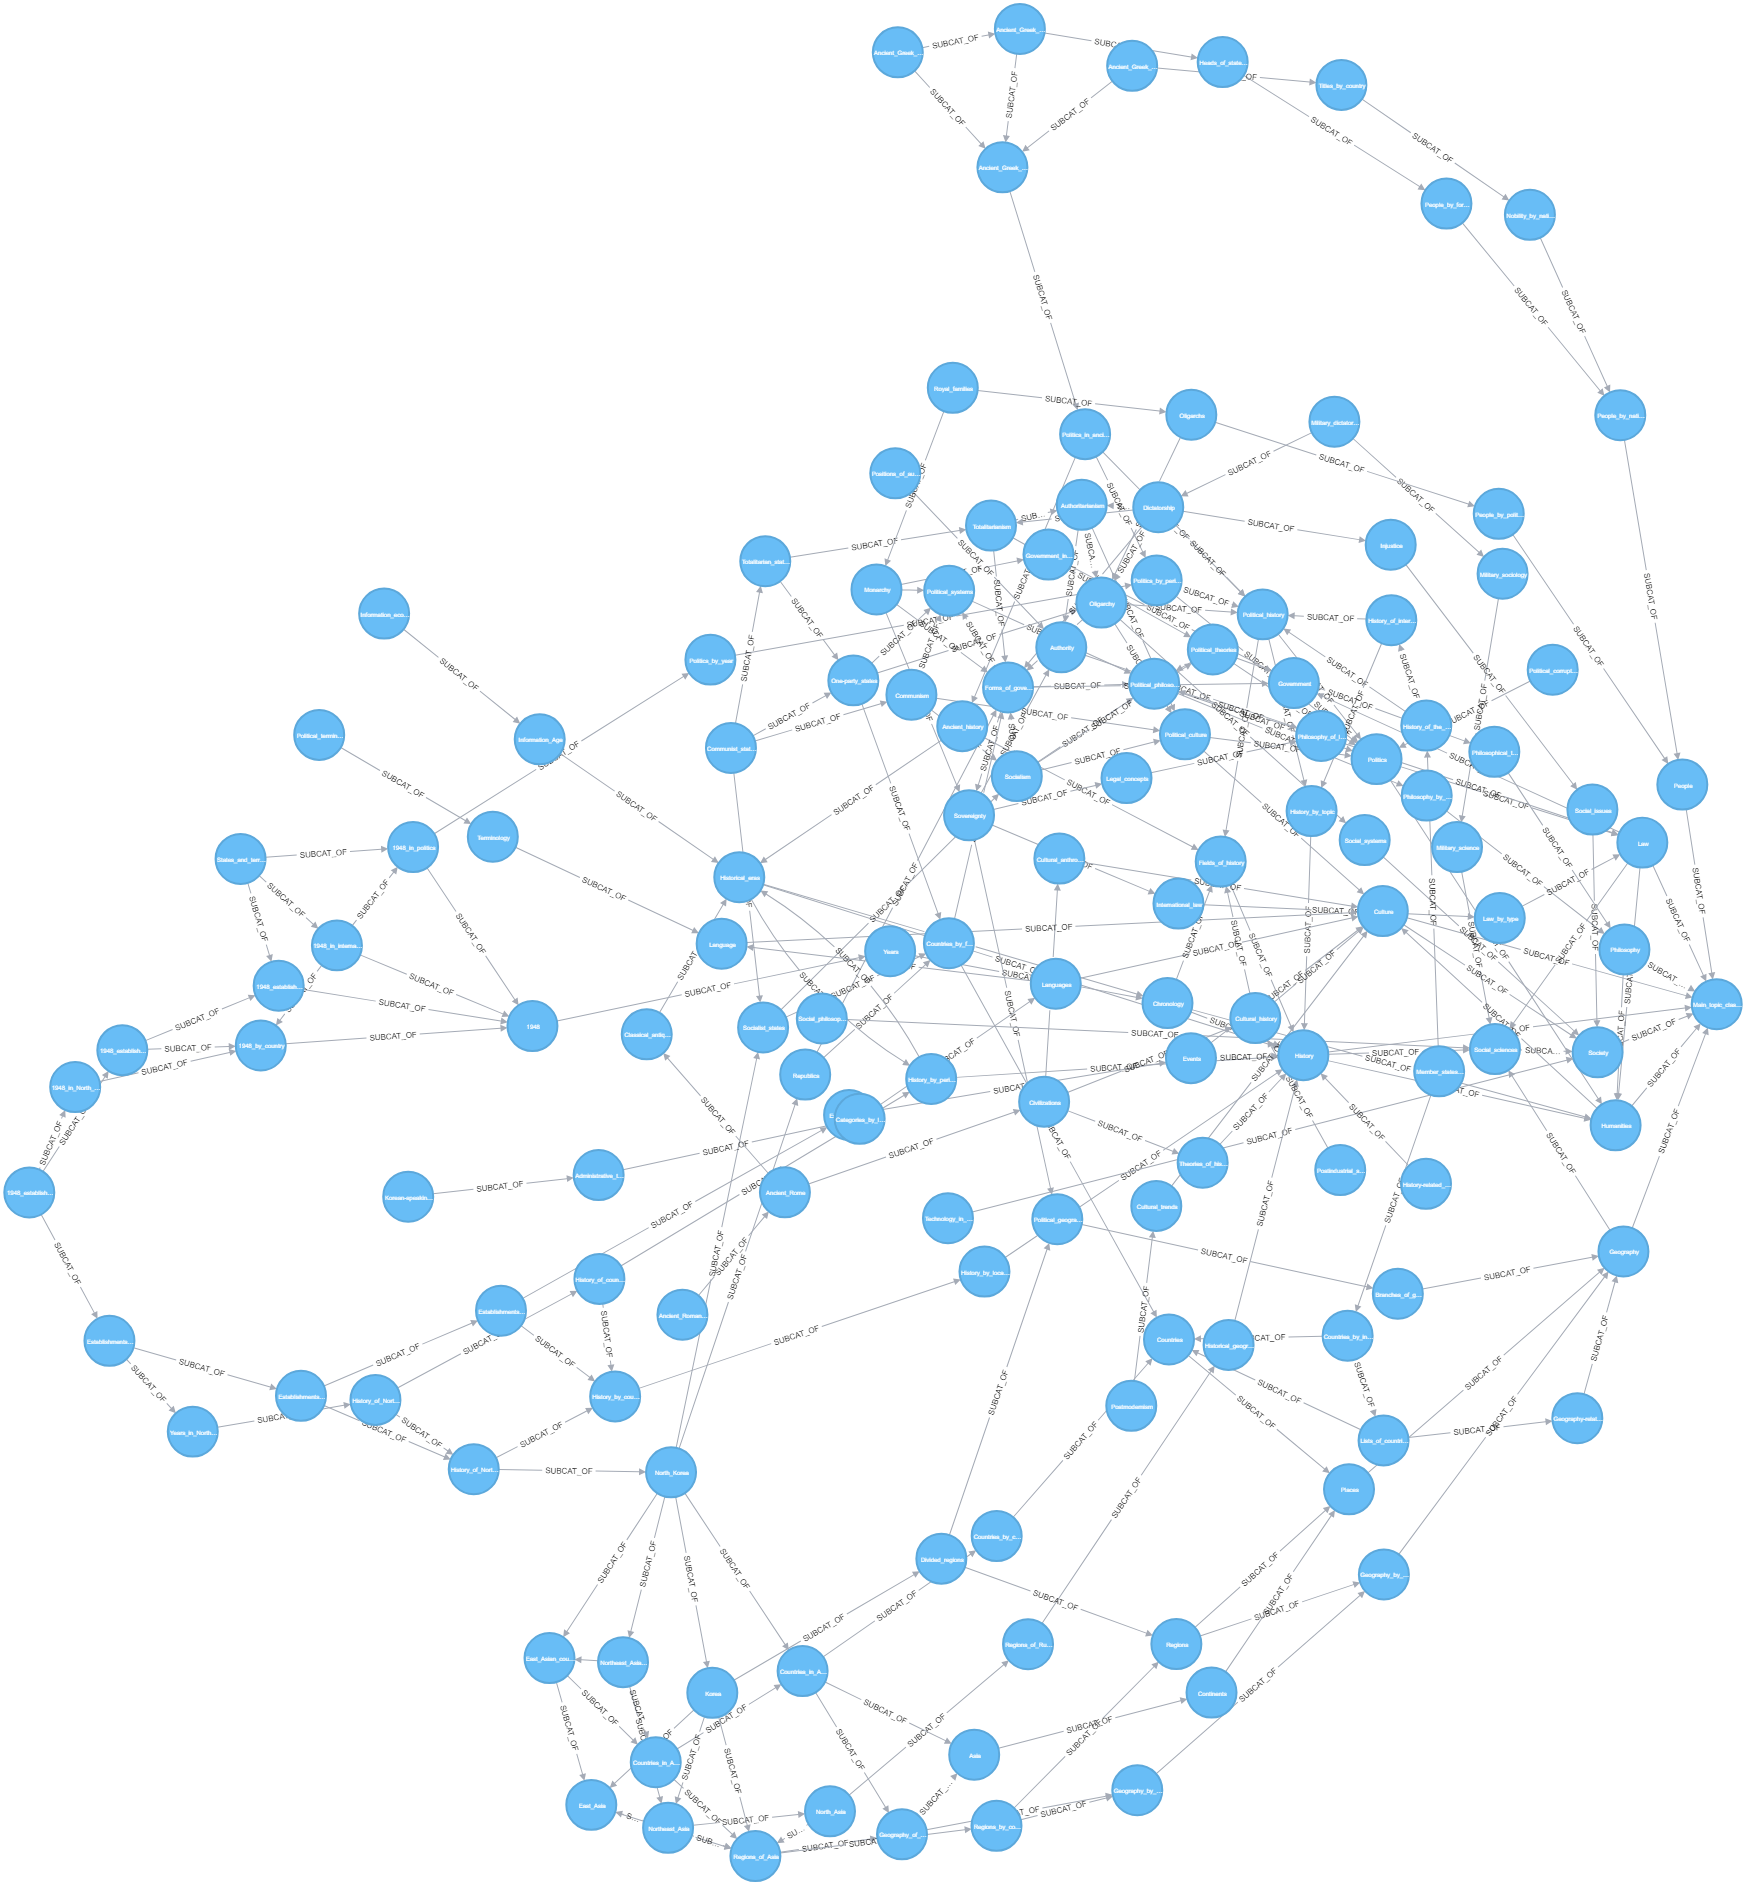
\includegraphics[width=\linewidth]{graph-example}
  \caption{An induced graph containing all shortest paths from the categories found and described in table \ref{tab:entities-categories} and ``Main topic classifications" (on the right of the graph)}
  \label{fig:graph-example}
\end{figure}


The vector generated for this example is shown in figure \ref{fig:final-classification-example}. Figure \ref{fig:final-classification-2} displays the absolute number of shortest paths used as features for the vector, while figure \ref{fig:final-classification-1} shows the same information normalized. Table \ref{tab:example-path-list} presents a random example of a path for each top-level category that contributed to the document representation.

\begin{figure}[htbp]
\centering
\begin{subfigure}{0.49\textwidth}
\centering
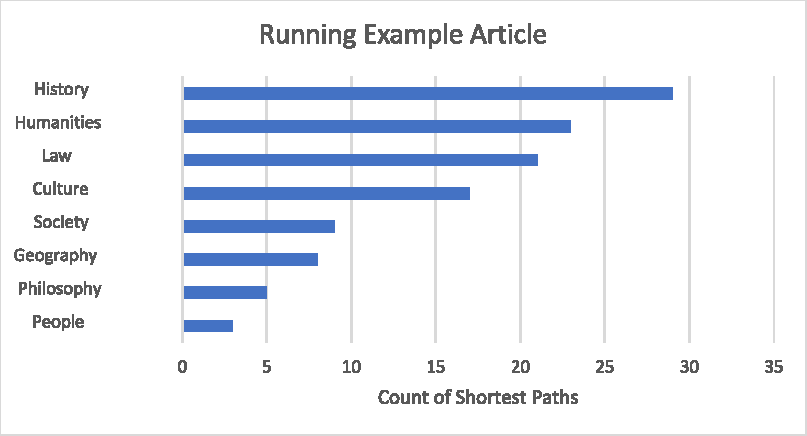
\includegraphics[width = \textwidth]{imgs/running_example_2}
\caption{Vector representation (count of shortest paths)}
\label{fig:final-classification-2}
\end{subfigure}
\begin{subfigure}{0.49\textwidth}
\centering
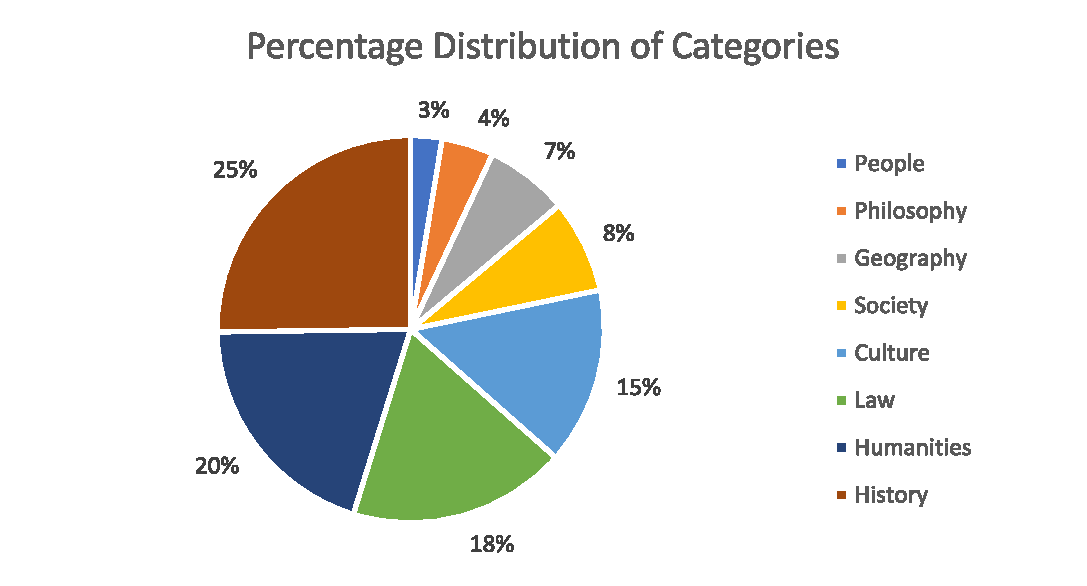
\includegraphics[width = \textwidth]{imgs/running_example_1}
\caption{Percentage distribution of categories}
\label{fig:final-classification-1}
\end{subfigure}
\caption{Final classification of the  running example according to our method}
\label{fig:final-classification-example}
\end{figure}



% Please add the following required packages to your document preamble:
% \usepackage{booktabs}
\begin{table}[H]
\caption{Example of a path for each top-level category that contributed to the document representation}
\label{tab:example-path-list}
\resizebox{\textwidth}{!}{%
\begin{tabular}{@{}ll@{}}
\toprule
Main Category & Shortest path example                                                                                                                                            \\ \midrule
History       & Theories of history $\rightarrow$ \textbf{History}                                                                                              \\
Humanities    & Political corruption $\rightarrow$ Politics $\rightarrow$ \textbf{Humanities}                                                                   \\
Law           & Political corruption $\rightarrow$ Politics $\rightarrow$ \textbf{Law}                                                                          \\
Culture       & Totalitarian states $\rightarrow$ Totalitarianism $\rightarrow$ Authoritarianism $\rightarrow$ Political culture $\rightarrow$ \textbf{Culture} \\
Society       & Military dictatorships $\rightarrow$ Dictatorship $\rightarrow$ Oligarchy $\rightarrow$ Social systems $\rightarrow$ \textbf{Society}           \\
Geography     & Korea $\rightarrow$ Divided regions $\rightarrow$ Political geography $\rightarrow$ Branches of geography $\rightarrow$ \textbf{Geography}      \\
Philosophy    & Forms of government $\rightarrow$ Political philosophy $\rightarrow$ Philosophy by topic $\rightarrow$ \textbf{Philosophy}                      \\
People        & Royal families $\rightarrow$ Oligarchs $\rightarrow$ People by political orientation $\rightarrow$ \textbf{People}                              \\ \bottomrule
\end{tabular}
}
\end{table}

For the article used in the running example, it can be inferred that it is strongly related to History, Humanities, Law, and Culture, and also has some weaker relatedness to Society, Geography, Philosophy, and People.


\section{\hspace*{3pt} Final Consideration}

This chapter presented the approach applied to the extraction of features and categorization of documents based on the \gls{wcg}. The method is based on three steps: extracting named entities from text, extracting categories associated with named entities, and finally representing and classifying the document.
The prime objective of this methodology is to generate a classification that can be used by humans, but that can also be applied in automated computational methods. For this reason, the result of classification was presented in two different formats. The vector of feature can be used in machine learning models and can help with automated such as search, retrieval, recommendation, and clustering of information. ON the other hand, the percentage distribution of categories is more tangible from a human point of view.
It is important to note that it is difficult to classify content in the Web in an arbitrary way since both in the documents and the Wikipedia structure there is fuzziness, ambiguity, inconsistency and lack of agreement of the contributors regarding some topics. For instance, at the moment of writing, there is no job role for Johann Sebastian Bach (the composer), the contributors cannot agree on what he should be known for. For this reason, the applied methodology does not define a single category for each textual resource, but a percentage distribution of each category concerning how much it contributes to the composition of the whole.